\chapter{FEM Verification}
\label{appx:FEM-verification}

This appendix provides the detailed process of verifying the structural analysis of the rotating climbing wall using both analytical calculations and Fusion 360 simulations for a cantilever beam setup.

\section{Introduction}
To ensure the structural integrity of the rotating climbing wall, a verification process was conducted by comparing the results from Fusion 360's static simulation with analytical calculations for a cantilever beam setup.

\section{Test Case Setup}
\subsection{Geometry}
A 76\,mm $\times$ 76\,mm $\times$ 2\,mm mild steel square tube, with a length of 2\,m, was used as the cantilever beam geometry for this verification.

\subsection{Material Properties}
The material properties applied for both the analytical calculations and the Fusion 360 simulations were as follows:
\begin{itemize}
    \item \textbf{Material:} Steel
    \item \textbf{Density:} $7.850 \times 10^{-6}$\,kg/mm\textsuperscript{3}
    \item \textbf{Young's Modulus:} 210\,GPa
    \item \textbf{Poisson's Ratio:} 0.30
    \item \textbf{Yield Strength:} 207\,MPa
    \item \textbf{Ultimate Tensile Strength:} 345\,MPa
\end{itemize}

\subsection{Boundary Conditions and Loading}
The cantilever beam was analyzed under the following conditions:
\begin{itemize}
    \item One end of the beam was fully fixed.
    \item A point load of 1000\,N was applied at the free end of the beam.
\end{itemize}

\section{Analytical Calculations}
The maximum bending stress and maximum deflection of the cantilever beam are calculated using the following formulas:

\begin{itemize}
    \item \textbf{Maximum Bending Stress:}
    \[
    \sigma_{\text{max}} = \frac{M \cdot c}{I} = \frac{P \cdot L \cdot c}{I} = \frac{1000\,\text{N} \times 2\,\text{m} \times 0.038\,\text{m}}{7.14 \times 10^{-6}\,\text{m}^4} = 140.56\,\text{MPa}
    \]
    \item \textbf{Maximum Deflection:}
    \[
    \delta_{\text{max}} = \frac{P \cdot L^3}{3 E I} = \frac{1000\,\text{N} \times 2^3\,\text{m}^3}{3 \times 210 \times 10^9\,\text{Pa} \times 7.14 \times 10^{-6}\,\text{m}^4} = 23.49\,\text{mm}
    \]
\end{itemize}

Where:

\begin{itemize}
    \item \( P = 1000\,\text{N} \) (applied load)
    \item \( L = 2\,\text{m} \) (length of the beam)
    \item \( c = \dfrac{76\,\text{mm}}{2} = 38\,\text{mm} = 0.038\,\text{m} \) (distance from the neutral axis to the outer fiber)
    \item \( I = \dfrac{(76\,\text{mm})^4 - (72\,\text{mm})^4}{12} = 7.14 \times 10^{-6}\,\text{m}^4 \) (second moment of area)
    \item \( E = 210 \times 10^9\,\text{Pa} \) (Young's modulus)
\end{itemize}

\section{Fusion 360 Simulation Setup}
The same material properties, boundary conditions, and load were applied in the Fusion 360 simulation as depicted in figures \ref{fig:max_stress} and \ref{fig:max_deflection}. A mesh sensitivity analysis was performed to ensure accurate capture of stress concentrations, particularly near the fixed end and the point load application.

\section{Results Comparison}
The results from the analytical calculations and Fusion 360 simulation were compared for maximum bending stress and deflection:

\begin{table}[H]
    \centering
    \begin{tabular}{|>{\centering\arraybackslash}p{0.35\linewidth}|>{\centering\arraybackslash}p{0.2\linewidth}|>{\centering\arraybackslash}p{0.2\linewidth}|>{\centering\arraybackslash}p{0.15\linewidth}|}
        \hline
        \textbf{Parameter} & \textbf{Analytical Result} & \textbf{Fusion 360 Result} & \textbf{Percentage Error (\%)} \\
        \hline
        Maximum Bending Stress (MPa) & 140.56 & 148.34 & 5.53 \\
        \hline
        Maximum Deflection (mm) & 23.49 & 23.62 & 0.57 \\
        \hline
    \end{tabular}
    \caption{Comparison of Analytical and Fusion 360 Simulation Results for Cantilever Beam}
    \label{tab:comparison_results}
\end{table}

\section{Conclusion}
The comparison demonstrates that the Fusion 360 simulation results align closely with the analytical calculations, with small percentage errors. This suggests that the simulation results are reliable for this application. Further refinement of simulation parameters, such as mesh density, could further improve the accuracy.

\begin{figure}[H]
    \centering
    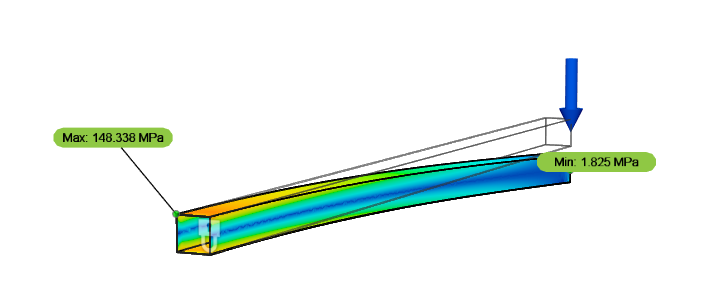
\includegraphics[width=1\textwidth]{figs/FEM/cantilever_beam_stress.png} 
    \caption{Fusion 360 Simulation Result: Maximum Bending Stress for Cantilever Beam}
    \label{fig:max_stress}
\end{figure}

\begin{figure}[H]
    \centering
    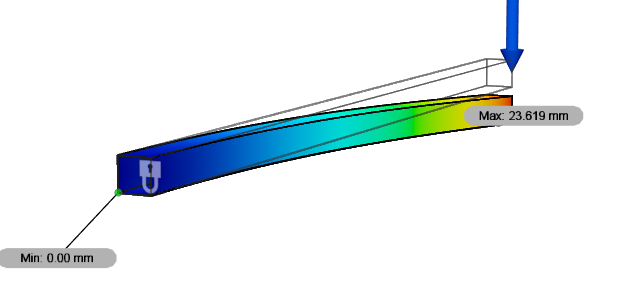
\includegraphics[width=1\textwidth]{figs/FEM/cantilever_beam_disp.png} 
    \caption{Fusion 360 Simulation Result: Maximum Deflection for Cantilever Beam}
    \label{fig:max_deflection}
\end{figure}
